\section{Control}
\subsection{Smoothing}
The purpose of smoothing is to create a new path without very sharp turns. The new path is also more like a continuous function and very likely also shorter in length. It is important to observe the smoothed path in order to find out whether the new path will move the robot into objects placed along the route.\\
To smooth out the path we use an algorithm that retains the start and goal while smoothing points in between. The first step is to initialise $y_i = x_i$ and then optimise equation \ref{eq:optimisesmooth} with respect to equations \ref{eq:equationsforsmooth1} and \ref{eq:equationsforsmooth2}.
\begin{gather}
minimise (x_i - y_i )^2 + \alpha(y_i - y_{i+1})^2
\label{eq:optimisesmooth} \\
y_i = y_i + \alpha(x_i - y_i)
\label{eq:equationsforsmooth1} \\
y_i = y_i + \beta(y_{i+1} + y_{i-1}-2y_i)
\label{eq:equationsforsmooth2}
\end{gather}
With $0\leq\alpha\leq1$ being how much we want to retain from the original path and $0\leq\beta\leq1$ being how much we want the path smoothed. This will results in something that looks like figure \ref{fig:pathsmooth}. The green circle shows the extend of the equations being optimised at three points.
\begin{figure}[H]
\centering
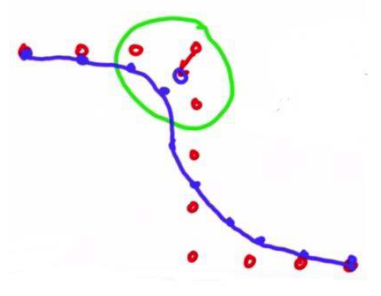
\includegraphics[width=0.4\textwidth]{billeder/pathsmoothed1}
\caption{Original points and a smoothed path}
\label{fig:pathsmooth}
\end{figure}

\subsection{PID Control}
PID is short for Proportional Integral Derivative. These three parts can be seen in equation \ref{eq:pid1}. Where $e(t) = u(t) - y(t)$, $u(t)$ is the control input, $x(t)$ is the input to the motor and $y(t)$ is the output from the motor as an example.
\begin{equation}
x(t) = K_p e(t) + K_i \int^t_0 e(\tau)d\tau + K_d\dfrac{de(t)}{dt}
\label{eq:pid1}
\end{equation}
Each part of the PID controller has a function. The P controller as seen in figure \ref{fig:pcontrol} has the responsibility of reducing the rise time and decreasing the steady-state error. An overshoot appears with larger $K_p$ values. $K_p$ is analogous to a gain.
\begin{figure}[H]
\centering
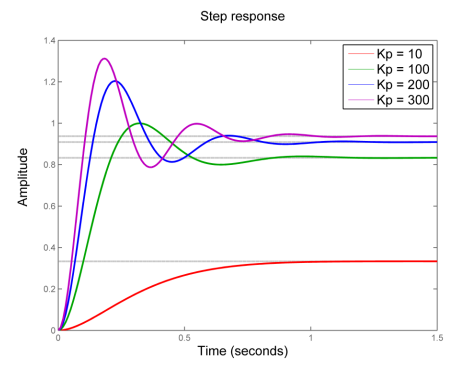
\includegraphics[width=0.5\textwidth]{billeder/pcontrol}
\caption{P Controller with different $K_p$ values}
\label{fig:pcontrol}
\end{figure}
The D controller is used along with the P controller to reduce the overshoot and the settling time. The D controller uses the slope of the function to reduce the error. This is seen in figure \ref{fig:pdcontrol}.
\begin{figure}[H]
\centering
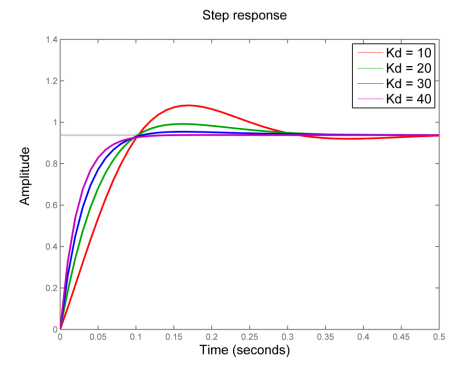
\includegraphics[width=0.5\textwidth]{billeder/pdcontrol}
\caption{PD Controller with different $K_d$ values}
\label{fig:pdcontrol}
\end{figure}
The I controller works with the integral of the error. This eliminates errors that persist over time. It will increase the overshoot and settling time, but fully eliminate the steady-state error. The is seen in figure \ref{fig:pidcontrol}.
\begin{figure}[H]
\centering
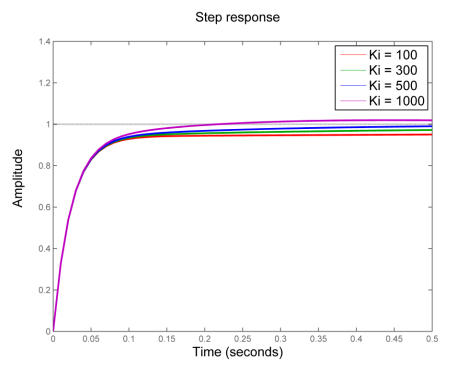
\includegraphics[width=0.5\textwidth]{billeder/pidcontrol}
\caption{PID Controller with different $K_i$ values}
\label{fig:pidcontrol}
\end{figure}
A collected table of all the effects of the three controllers can be seen in table \ref{tab:PIDcontrol}.
\begin{table}[H]
	\centering
    \begin{tabular}{|l|l|l|l|l|}
    \hline
    ~  & Rise Time    & Overshoot & Settling time & Steady-State Error \\ \hline
    $K_p$ & Decreases    & Increases & Small Change  & Decrease           \\ \hline
    $K_i$ & Decreases    & Increases & Increases     & Eliminate          \\ \hline
    $K_d$ & Small Change & Decreases & Decreases     & No Change          \\ \hline
    \end{tabular}
    \caption{PID Control effects}
    \label{tab:PIDcontrol}
\end{table}
A way to find good values for the $K_p$, $K_i$ and $K_p$ terms is to use twiddle. Twiddle or Coordinate descent works out a local minimum by doing a line search through different values of the controllers. The values can also be found in a manual way by tuning the values as you work out what is subjectively the best controller.
%------------------------------------------------